\chapter{Theory}
Following is a brief introduction to some of the aspects that affects the solution, and should be among the things considered when developing a commercial application.

\section{Hardware}
\subsection{Camera}
The camera specifications and performance directly affects the results. It is the source of input data for the computer vision software, and it may also be the output, which will be the case when the PTZ is controlled by the software.

Some cameras support extra applications that run in their firmware, which can for example track moving objects and "fence" an area so that any objects who enter a region of interest, will raise an alarm.
The CPU and memory of embedded systems is constraining, so any complex applications may be better off being executed on a stand-alone computer.

\subsubsection{Resolution and Field of view}
Resolution and Field of view are related such that an increased field of view leads to a lower amount of pixels available to distinguish objects. Modern image sensors come with capabilities of capturing 1920x1080 pixel images, whilst older image sensors may capture 320x240 pixel images.
The field of view is a function of the optical objective as well as the size of the image sensor, and their distances in relation to each other.

\subsubsection{Pan, Tilt and Zoom}
Many modern CCTV cameras come with motors that can pan and tilt the camera, as well as optical and digital zoom functionality. Their ability to pan, tilt and zoom have uses for scanning a large area, as well as investigating small areas in detail.
The speed and accuracy of which the pan, tilt and zoom can be manipulated may be of importance in some applications.

\subsubsection{Focus}
If light from an object converges as much as possible, it is considered in focus. Would the light rather diverge, it is considered out of focus. This leads to blurring of the object or scene in question.
Many cameras come with automatic focus that will try to adjust the focus so that a target object becomes in focus. The focus is then controlled by either an ultrasonic motor or a stepper motor.

\subsubsection{Iris}
The iris determines how much light enters the camera, and it is also a factor that can determine the focus range of a camera. An open iris leads to larger amounts of light and thus works better in low-light conditions, but the depth of field gets smaller.
The amount of light that enters and hits the image sensor also determines how long the iris should be kept open before a picture is fully captured, and less light means that it will need to stay open longer, which in turn leads to motion blur if an object is in motion.
Many cameras come with automatic iris control, that will try to adjust the iris so that the picture does not get too bright or too dark. This is also called DC-iris.
Axis Communications have introduced precise iris control to some cameras, known as P-iris, which provides improvements to contrast, clarity, resolution and depth of field beyond the DC-iris.

\begin{figure}[ht]
    \centering
    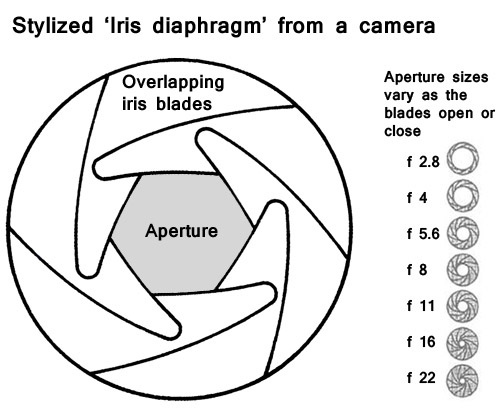
\includegraphics[width=0.8\textwidth]{7228218072_042541190a.jpg}
    \caption{Iris. Source: Online \citet{iris15}}
    \label{fig:cfs_simple_new}
\end{figure}
\FloatBarrier

\begin{figure}[ht]
    \centering
    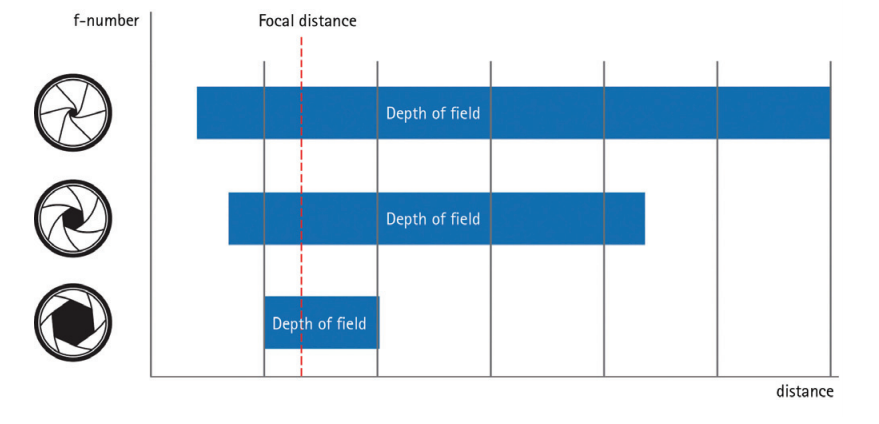
\includegraphics[width=1.0\textwidth]{iris_dof_axis.png}
    \caption{Correlation between iris opening and depth of field. Source: Online \citet{axispiris15}}
    \label{fig:cfs_simple_new}
\end{figure}
\FloatBarrier

\subsubsection{Frame Rate}
The number of frames that can be captured per second determines the frame rate, and is usually used to give the illusion of movement in a movie. The human eye usually sees 25 frames per second as a movie, any less will deteriorate the experience of watching a movie.
A large amount of frames per second requires a multiple of the image resolution of bandwidth to transfer the images to a viewer.
When it comes to CCTV cameras for surveillance, frame rate of stored movies are reduced to allow for longer storage of material. 

\subsubsection{Image Quality}
The quality of an image is related to the quality of the optics, quality of the image sensor and amount of light available at a scene, as well as the firmware which translates the impression to data, in addition to other factors.
Modern image sensors can also adjust the sensitivity of the sensor so that previously dark scenes look brighter, at the cost of increased pixel noise.
A full overview over the factors that affect image quality can be found at \citep{imatest15}.

\subsubsection{Camera Interface}
Which interface that is supported for transferring images is an important factor to consider, both to reduce cost and increase performance.
Some of the most used interfaces include USB, FireWire and Ethernet. It is also possible to find CCTV cameras that rely on Wi-Fi, but these are prone to intermittent frame drops if environmental conditions blocks the signal.
The most cost-effective method of interfacing a camera is through Ethernet, as the cables are cheap and the Ethernet standard supports a large amount of data. Maximum theoretical capacity of the most common Ethernet link is 100 Mbit per second, but this is quickly shifting to 1000 Mbit per second for modern Ethernet.

\subsection{Data transmission}
A function of the camera hardware and firmware, the camera interface and path of transmission as well as any processing on the way, several aspects will affect data transmission from the image sensor to the screen. An unfortunate side-effect of data transmission is that an image lags after the actual event got captured, and we commonly call this for latency.

\begin{figure}[ht]
    \centering
    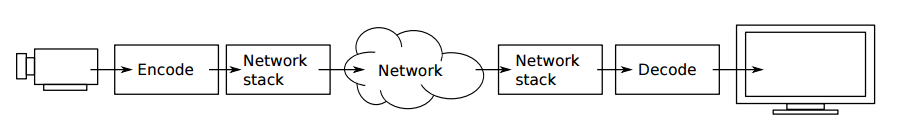
\includegraphics[width=1.0\textwidth]{svensson13_network.png}
    \caption{Diagram of data through an IP network. Source: \citet{svensson13}}
    \label{fig:cfs_simple_new}
\end{figure}
\FloatBarrier

\subsection{Glyph visibility}
The glyph symbol, if it is going to be used outdoors or in difficult lightning situations, may have reduced visibility when light hits the glyph from some angles. The angle of light from a sun hitting a glyph can change with the time of the year, time of the day and any man-made sources of light. The method of drawing and displaying the symbol is important to consider.
Using a thin translucent plastic sheet to laminate a paper print of the glyph may give specular reflections that appear white. The specular reflection is a function of the glossiness of a surface. Thus to increase reliability of glyph detection, the surface should have a low glossiness.

\begin{figure}[ht]
    \centering
    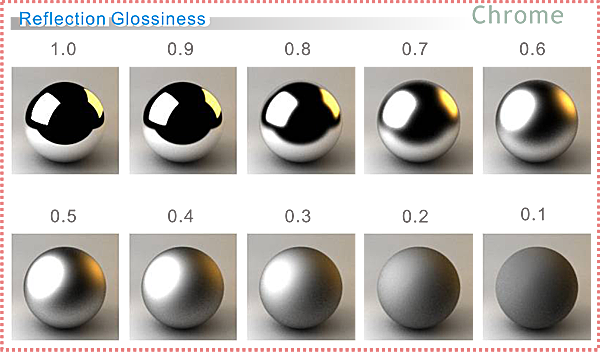
\includegraphics[width=0.8\textwidth]{reflection_layer_in_vray_for_sketchup_4.png}
    \caption{Glossiness and its change on reflection as shown in raytracing software. Source: Online \citet{gloss15}}
    \label{fig:cfs_simple_new}
\end{figure}
\FloatBarrier

\subsection{Computing platform}
The processing of images may be done by humans, in which the image is sent directly to a screen. In cases where we want to use machine vision algorithms, a general purpose computer is typically doing this job.

The computing platform is connected to the camera, and it gathers images which is then processed by a computer program.

Computer performance using a central processing unit is steadily increasing as new technologies evolve, but a relatively new method uses a graphical processing unit to accelerate application code. This allows for highly parallel execution of code, that may for some algorithms, speed up their execution and in turn speed up the program.

\section{Software}
\subsection{Threading}
In order to allow several different threads to run simultaneously, the operating system supports threads. It is also possible to delegate a thread to a specific computing core in a central processing unit, if there are more. This have both advantages and disadvantages.

Advantages include the ability for the computer to use idle processing time, and also allow for blocking functions to run in seperate threads to allow the main thread to continue running.

Disadvantages include possibilities of interfering with each other if they share memory, and it is also notoriously challenging to write good multi threaded applications, which in turn may lead to the program not functioning as expected.

\begin{figure}[ht]
    \centering
    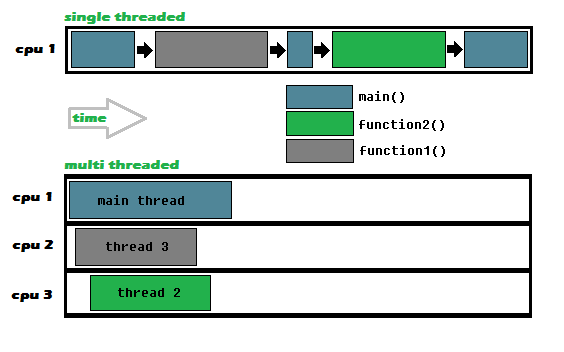
\includegraphics[width=1.0\textwidth]{multithreading.png}
    \caption{Singlethread versus multithread execution. Source: Online \citet{multithreadingcpp15}}
    \label{fig:cfs_simple_new}
\end{figure}
\FloatBarrier

Modern central processing units contains several computing cores, which can run their own threads if the programmer wishes. The number of computing cores usually range from one to eight in personal computers.

\subsection{Heterogenous computing}
Systems that utilize dissimilar processing cores are known as heterogenous computing systems. Not only do they have the benefit of several processing cores, they also bring the benefit of having dissimilar processing units that work differently and are better at handling specific tasks.

Heterogenous System Architecture can be used to integrate central processing units and graphical processing units, the alternative is to use a parallel computing platform like OpenCL or CUDA that relieves the programmer from having to move data between the processing units themselves.

\begin{figure}[ht]
    \centering
    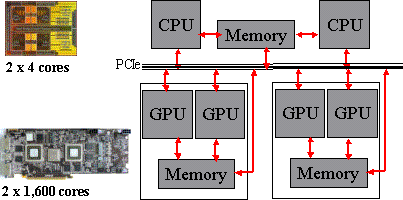
\includegraphics[width=0.8\textwidth]{cpu-gpu.png}
    \caption{Conceptual overview of a heterogeneous system with CPU and GPU cores. Source: Online \citet{cpugpu13}}
    \label{fig:cfs_simple_new}
\end{figure}
\FloatBarrier

\subsubsection{CUDA}
The NVIDIA Corporation released the CUDA platform in June 2007, and is a parallel computing platform that only works with NVIDIA graphic cards. It can also utilize OpenCL. Language bindings exist for many programming languages, and it provides both low-level and high-level APIs.

\begin{figure}[ht]
    \centering
    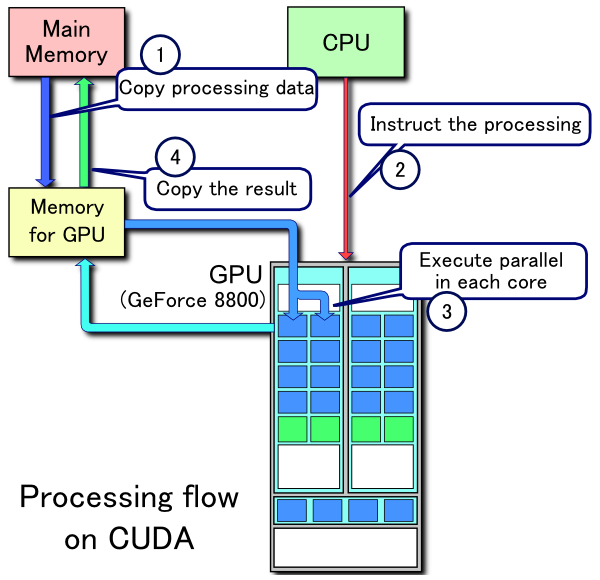
\includegraphics[width=0.8\textwidth]{CUDA_processing_flow_(En).PNG}
    \caption{CUDA processing flow. Source: Online \citet{wikicuda15}}
    \label{fig:cfs_simple_new}
\end{figure}
\FloatBarrier

\subsubsection{OpenCL}
Apple Inc. authored a language and an API that executes across central processing units, graphical processing units and other processors in August 2009. This is now maintained by the Khronos Group, which is a non-profit consortium that develops open standards for graphics, media and parallel computation. They also maintain OpenGL, which sees great use in 3D applications.

OpenCL sees all computing devices, not only the graphical processing units, and a key feature of it is to be portable and run on any system that conforms to the standard.

A comprehensive study by \citep{fang11} in 2011 compared CUDA to OpenCL, and the findings suggests that CUDA performs 30 percent faster than OpenCL when a program is directly translated between the two platforms. However, the conclusion is that there are no reason for OpenCL to perform worse than CUDA under a fair comparison, and OpenCL is considered a good alternative to CUDA.

\subsection{Machine vision}
Machine vision is a relatively new field that uses image capture and analysis for automating tasks. It sees wide use in industrial manufacturing for quality control and process automation, and also in more recent times, autonomous vehicles.

Implementing machine vision in software is often done by using vision libraries, and one well-known is the Open Source Computer Vision Library. The short-form is OpenCV, and it is currently on its third release, being maintained by a russian company named Itseez and developed by contributors all around the world.

OpenCV 3.0 gold release was made available in 4th of June 2015. It supports OpenCL using its transparent API, and support for CUDA was developed in 2010. Both the OpenCL and CUDA support is still under active development.

\begin{figure}[ht]
    \centering
    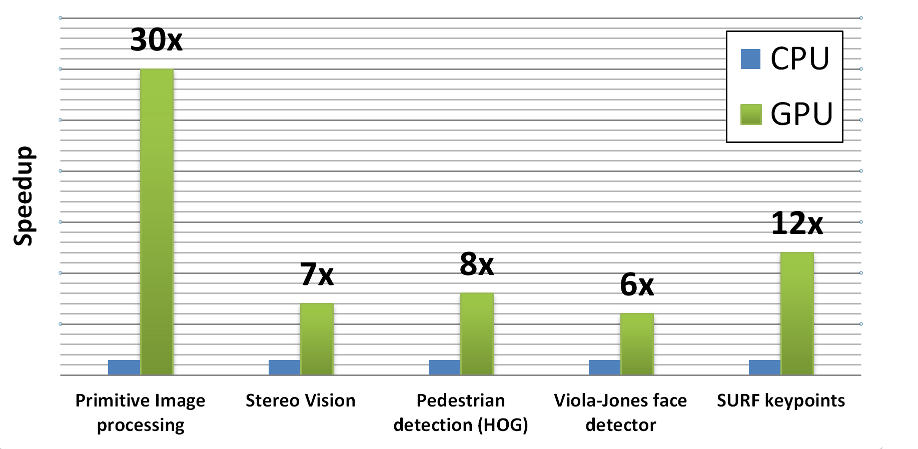
\includegraphics[width=0.8\textwidth]{perfcudavscpuopencv.png}
    \caption{Performance speedups when using CUDA and a GPU. Source: Online \citet{opencvcuda15}}
    \label{fig:cfs_simple_new}
\end{figure}
\FloatBarrier


\subsection{Linux}